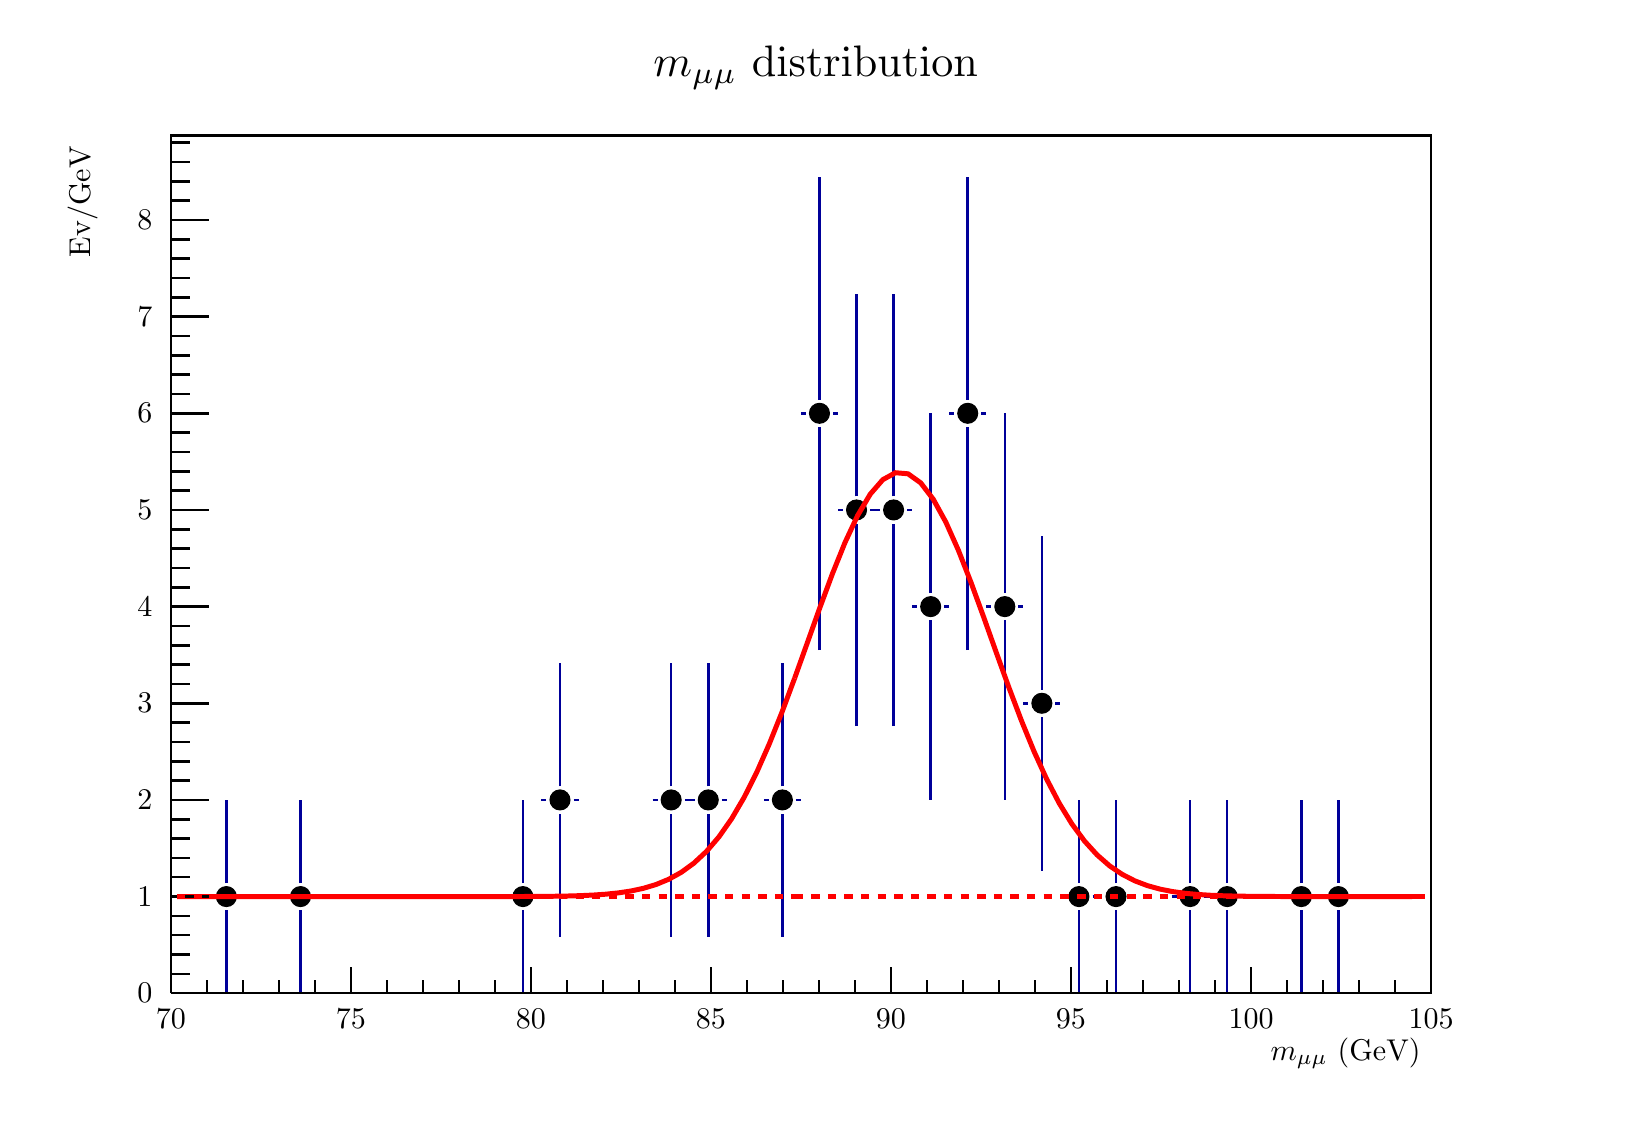
\begin{tikzpicture}
\pgfdeclareplotmark{cross} {
\pgfpathmoveto{\pgfpoint{-0.3\pgfplotmarksize}{\pgfplotmarksize}}
\pgfpathlineto{\pgfpoint{+0.3\pgfplotmarksize}{\pgfplotmarksize}}
\pgfpathlineto{\pgfpoint{+0.3\pgfplotmarksize}{0.3\pgfplotmarksize}}
\pgfpathlineto{\pgfpoint{+1\pgfplotmarksize}{0.3\pgfplotmarksize}}
\pgfpathlineto{\pgfpoint{+1\pgfplotmarksize}{-0.3\pgfplotmarksize}}
\pgfpathlineto{\pgfpoint{+0.3\pgfplotmarksize}{-0.3\pgfplotmarksize}}
\pgfpathlineto{\pgfpoint{+0.3\pgfplotmarksize}{-1.\pgfplotmarksize}}
\pgfpathlineto{\pgfpoint{-0.3\pgfplotmarksize}{-1.\pgfplotmarksize}}
\pgfpathlineto{\pgfpoint{-0.3\pgfplotmarksize}{-0.3\pgfplotmarksize}}
\pgfpathlineto{\pgfpoint{-1.\pgfplotmarksize}{-0.3\pgfplotmarksize}}
\pgfpathlineto{\pgfpoint{-1.\pgfplotmarksize}{0.3\pgfplotmarksize}}
\pgfpathlineto{\pgfpoint{-0.3\pgfplotmarksize}{0.3\pgfplotmarksize}}
\pgfpathclose
\pgfusepathqstroke
}
\pgfdeclareplotmark{cross*} {
\pgfpathmoveto{\pgfpoint{-0.3\pgfplotmarksize}{\pgfplotmarksize}}
\pgfpathlineto{\pgfpoint{+0.3\pgfplotmarksize}{\pgfplotmarksize}}
\pgfpathlineto{\pgfpoint{+0.3\pgfplotmarksize}{0.3\pgfplotmarksize}}
\pgfpathlineto{\pgfpoint{+1\pgfplotmarksize}{0.3\pgfplotmarksize}}
\pgfpathlineto{\pgfpoint{+1\pgfplotmarksize}{-0.3\pgfplotmarksize}}
\pgfpathlineto{\pgfpoint{+0.3\pgfplotmarksize}{-0.3\pgfplotmarksize}}
\pgfpathlineto{\pgfpoint{+0.3\pgfplotmarksize}{-1.\pgfplotmarksize}}
\pgfpathlineto{\pgfpoint{-0.3\pgfplotmarksize}{-1.\pgfplotmarksize}}
\pgfpathlineto{\pgfpoint{-0.3\pgfplotmarksize}{-0.3\pgfplotmarksize}}
\pgfpathlineto{\pgfpoint{-1.\pgfplotmarksize}{-0.3\pgfplotmarksize}}
\pgfpathlineto{\pgfpoint{-1.\pgfplotmarksize}{0.3\pgfplotmarksize}}
\pgfpathlineto{\pgfpoint{-0.3\pgfplotmarksize}{0.3\pgfplotmarksize}}
\pgfpathclose
\pgfusepathqfillstroke
}
\pgfdeclareplotmark{newstar} {
\pgfpathmoveto{\pgfqpoint{0pt}{\pgfplotmarksize}}
\pgfpathlineto{\pgfqpointpolar{44}{0.5\pgfplotmarksize}}
\pgfpathlineto{\pgfqpointpolar{18}{\pgfplotmarksize}}
\pgfpathlineto{\pgfqpointpolar{-20}{0.5\pgfplotmarksize}}
\pgfpathlineto{\pgfqpointpolar{-54}{\pgfplotmarksize}}
\pgfpathlineto{\pgfqpointpolar{-90}{0.5\pgfplotmarksize}}
\pgfpathlineto{\pgfqpointpolar{234}{\pgfplotmarksize}}
\pgfpathlineto{\pgfqpointpolar{198}{0.5\pgfplotmarksize}}
\pgfpathlineto{\pgfqpointpolar{162}{\pgfplotmarksize}}
\pgfpathlineto{\pgfqpointpolar{134}{0.5\pgfplotmarksize}}
\pgfpathclose
\pgfusepathqstroke
}
\pgfdeclareplotmark{newstar*} {
\pgfpathmoveto{\pgfqpoint{0pt}{\pgfplotmarksize}}
\pgfpathlineto{\pgfqpointpolar{44}{0.5\pgfplotmarksize}}
\pgfpathlineto{\pgfqpointpolar{18}{\pgfplotmarksize}}
\pgfpathlineto{\pgfqpointpolar{-20}{0.5\pgfplotmarksize}}
\pgfpathlineto{\pgfqpointpolar{-54}{\pgfplotmarksize}}
\pgfpathlineto{\pgfqpointpolar{-90}{0.5\pgfplotmarksize}}
\pgfpathlineto{\pgfqpointpolar{234}{\pgfplotmarksize}}
\pgfpathlineto{\pgfqpointpolar{198}{0.5\pgfplotmarksize}}
\pgfpathlineto{\pgfqpointpolar{162}{\pgfplotmarksize}}
\pgfpathlineto{\pgfqpointpolar{134}{0.5\pgfplotmarksize}}
\pgfpathclose
\pgfusepathqfillstroke
}
\definecolor{c}{rgb}{1,1,1};
\draw [color=c, fill=c] (0,0) rectangle (20,13.6207);
\draw [color=c, fill=c] (1.81034,1.36494) rectangle (17.8161,12.2557);
\definecolor{c}{rgb}{0,0,0};
\draw [c,line width=0.9] (1.81034,1.36494) -- (1.81034,12.2557) -- (17.8161,12.2557) -- (17.8161,1.36494) -- (1.81034,1.36494);
\definecolor{c}{rgb}{1,1,1};
\draw [color=c, fill=c] (1.81034,1.36494) rectangle (17.8161,12.2557);
\definecolor{c}{rgb}{0,0,0};
\draw [c,line width=0.9] (1.81034,1.36494) -- (1.81034,12.2557) -- (17.8161,12.2557) -- (17.8161,1.36494) -- (1.81034,1.36494);
\definecolor{c}{rgb}{0,0,0.6};
\draw [c,line width=0.9] (2.51648,1.36494) -- (2.51648,2.42008);
\draw [c,line width=0.9] (2.51648,2.76491) -- (2.51648,3.82005);
\draw [c,line width=0.9] (2.2811,2.5925) -- (2.34407,2.5925);
\draw [c,line width=0.9] (2.68889,2.5925) -- (2.75186,2.5925);
\definecolor{c}{rgb}{0,0,0};
\foreach \P in {(2.51648,2.5925)}{\draw[mark options={color=c,fill=c},mark size=3.603604pt,mark=*] plot coordinates {\P};}
\definecolor{c}{rgb}{0,0,0.6};
\draw [c,line width=0.9] (3.458,1.36494) -- (3.458,2.42008);
\draw [c,line width=0.9] (3.458,2.76491) -- (3.458,3.82005);
\draw [c,line width=0.9] (3.22262,2.5925) -- (3.28558,2.5925);
\draw [c,line width=0.9] (3.63041,2.5925) -- (3.69337,2.5925);
\definecolor{c}{rgb}{0,0,0};
\foreach \P in {(3.458,2.5925)}{\draw[mark options={color=c,fill=c},mark size=3.603604pt,mark=*] plot coordinates {\P};}
\definecolor{c}{rgb}{0,0,0.6};
\draw [c,line width=0.9] (6.28254,1.36494) -- (6.28254,2.42008);
\draw [c,line width=0.9] (6.28254,2.76491) -- (6.28254,3.82005);
\draw [c,line width=0.9] (6.04716,2.5925) -- (6.11013,2.5925);
\draw [c,line width=0.9] (6.45495,2.5925) -- (6.51792,2.5925);
\definecolor{c}{rgb}{0,0,0};
\foreach \P in {(6.28254,2.5925)}{\draw[mark options={color=c,fill=c},mark size=3.603604pt,mark=*] plot coordinates {\P};}
\definecolor{c}{rgb}{0,0,0.6};
\draw [c,line width=0.9] (6.7533,2.08403) -- (6.7533,3.64763);
\draw [c,line width=0.9] (6.7533,3.99246) -- (6.7533,5.55607);
\draw [c,line width=0.9] (6.51792,3.82005) -- (6.58088,3.82005);
\draw [c,line width=0.9] (6.92571,3.82005) -- (6.98867,3.82005);
\definecolor{c}{rgb}{0,0,0};
\foreach \P in {(6.7533,3.82005)}{\draw[mark options={color=c,fill=c},mark size=3.603604pt,mark=*] plot coordinates {\P};}
\definecolor{c}{rgb}{0,0,0.6};
\draw [c,line width=0.9] (8.16557,2.08403) -- (8.16557,3.64763);
\draw [c,line width=0.9] (8.16557,3.99246) -- (8.16557,5.55607);
\draw [c,line width=0.9] (7.93019,3.82005) -- (7.99315,3.82005);
\draw [c,line width=0.9] (8.33798,3.82005) -- (8.40095,3.82005);
\definecolor{c}{rgb}{0,0,0};
\foreach \P in {(8.16557,3.82005)}{\draw[mark options={color=c,fill=c},mark size=3.603604pt,mark=*] plot coordinates {\P};}
\definecolor{c}{rgb}{0,0,0.6};
\draw [c,line width=0.9] (8.63632,2.08403) -- (8.63632,3.64763);
\draw [c,line width=0.9] (8.63632,3.99246) -- (8.63632,5.55607);
\draw [c,line width=0.9] (8.40095,3.82005) -- (8.46391,3.82005);
\draw [c,line width=0.9] (8.80874,3.82005) -- (8.8717,3.82005);
\definecolor{c}{rgb}{0,0,0};
\foreach \P in {(8.63632,3.82005)}{\draw[mark options={color=c,fill=c},mark size=3.603604pt,mark=*] plot coordinates {\P};}
\definecolor{c}{rgb}{0,0,0.6};
\draw [c,line width=0.9] (9.57784,2.08403) -- (9.57784,3.64763);
\draw [c,line width=0.9] (9.57784,3.99246) -- (9.57784,5.55607);
\draw [c,line width=0.9] (9.34246,3.82005) -- (9.40543,3.82005);
\draw [c,line width=0.9] (9.75025,3.82005) -- (9.81322,3.82005);
\definecolor{c}{rgb}{0,0,0};
\foreach \P in {(9.57784,3.82005)}{\draw[mark options={color=c,fill=c},mark size=3.603604pt,mark=*] plot coordinates {\P};}
\definecolor{c}{rgb}{0,0,0.6};
\draw [c,line width=0.9] (10.0486,5.72338) -- (10.0486,8.55785);
\draw [c,line width=0.9] (10.0486,8.90267) -- (10.0486,11.7371);
\draw [c,line width=0.9] (9.81322,8.73026) -- (9.87618,8.73026);
\draw [c,line width=0.9] (10.221,8.73026) -- (10.284,8.73026);
\definecolor{c}{rgb}{0,0,0};
\foreach \P in {(10.0486,8.73026)}{\draw[mark options={color=c,fill=c},mark size=3.603604pt,mark=*] plot coordinates {\P};}
\definecolor{c}{rgb}{0,0,0.6};
\draw [c,line width=0.9] (10.5194,4.75781) -- (10.5194,7.33029);
\draw [c,line width=0.9] (10.5194,7.67512) -- (10.5194,10.2476);
\draw [c,line width=0.9] (10.284,7.50271) -- (10.3469,7.50271);
\draw [c,line width=0.9] (10.6918,7.50271) -- (10.7547,7.50271);
\definecolor{c}{rgb}{0,0,0};
\foreach \P in {(10.5194,7.50271)}{\draw[mark options={color=c,fill=c},mark size=3.603604pt,mark=*] plot coordinates {\P};}
\definecolor{c}{rgb}{0,0,0.6};
\draw [c,line width=0.9] (10.9901,4.75781) -- (10.9901,7.33029);
\draw [c,line width=0.9] (10.9901,7.67512) -- (10.9901,10.2476);
\draw [c,line width=0.9] (10.7547,7.50271) -- (10.8177,7.50271);
\draw [c,line width=0.9] (11.1625,7.50271) -- (11.2255,7.50271);
\definecolor{c}{rgb}{0,0,0};
\foreach \P in {(10.9901,7.50271)}{\draw[mark options={color=c,fill=c},mark size=3.603604pt,mark=*] plot coordinates {\P};}
\definecolor{c}{rgb}{0,0,0.6};
\draw [c,line width=0.9] (11.4609,3.82005) -- (11.4609,6.10274);
\draw [c,line width=0.9] (11.4609,6.44757) -- (11.4609,8.73026);
\draw [c,line width=0.9] (11.2255,6.27515) -- (11.2885,6.27515);
\draw [c,line width=0.9] (11.6333,6.27515) -- (11.6962,6.27515);
\definecolor{c}{rgb}{0,0,0};
\foreach \P in {(11.4609,6.27515)}{\draw[mark options={color=c,fill=c},mark size=3.603604pt,mark=*] plot coordinates {\P};}
\definecolor{c}{rgb}{0,0,0.6};
\draw [c,line width=0.9] (11.9316,5.72338) -- (11.9316,8.55785);
\draw [c,line width=0.9] (11.9316,8.90267) -- (11.9316,11.7371);
\draw [c,line width=0.9] (11.6962,8.73026) -- (11.7592,8.73026);
\draw [c,line width=0.9] (12.104,8.73026) -- (12.167,8.73026);
\definecolor{c}{rgb}{0,0,0};
\foreach \P in {(11.9316,8.73026)}{\draw[mark options={color=c,fill=c},mark size=3.603604pt,mark=*] plot coordinates {\P};}
\definecolor{c}{rgb}{0,0,0.6};
\draw [c,line width=0.9] (12.4024,3.82005) -- (12.4024,6.10274);
\draw [c,line width=0.9] (12.4024,6.44757) -- (12.4024,8.73026);
\draw [c,line width=0.9] (12.167,6.27515) -- (12.23,6.27515);
\draw [c,line width=0.9] (12.5748,6.27515) -- (12.6378,6.27515);
\definecolor{c}{rgb}{0,0,0};
\foreach \P in {(12.4024,6.27515)}{\draw[mark options={color=c,fill=c},mark size=3.603604pt,mark=*] plot coordinates {\P};}
\definecolor{c}{rgb}{0,0,0.6};
\draw [c,line width=0.9] (12.8731,2.92142) -- (12.8731,4.87519);
\draw [c,line width=0.9] (12.8731,5.22001) -- (12.8731,7.17378);
\draw [c,line width=0.9] (12.6378,5.0476) -- (12.7007,5.0476);
\draw [c,line width=0.9] (13.0456,5.0476) -- (13.1085,5.0476);
\definecolor{c}{rgb}{0,0,0};
\foreach \P in {(12.8731,5.0476)}{\draw[mark options={color=c,fill=c},mark size=3.603604pt,mark=*] plot coordinates {\P};}
\definecolor{c}{rgb}{0,0,0.6};
\draw [c,line width=0.9] (13.3439,1.36494) -- (13.3439,2.42008);
\draw [c,line width=0.9] (13.3439,2.76491) -- (13.3439,3.82005);
\draw [c,line width=0.9] (13.1085,2.5925) -- (13.1715,2.5925);
\draw [c,line width=0.9] (13.5163,2.5925) -- (13.5793,2.5925);
\definecolor{c}{rgb}{0,0,0};
\foreach \P in {(13.3439,2.5925)}{\draw[mark options={color=c,fill=c},mark size=3.603604pt,mark=*] plot coordinates {\P};}
\definecolor{c}{rgb}{0,0,0.6};
\draw [c,line width=0.9] (13.8147,1.36494) -- (13.8147,2.42008);
\draw [c,line width=0.9] (13.8147,2.76491) -- (13.8147,3.82005);
\draw [c,line width=0.9] (13.5793,2.5925) -- (13.6422,2.5925);
\draw [c,line width=0.9] (13.9871,2.5925) -- (14.05,2.5925);
\definecolor{c}{rgb}{0,0,0};
\foreach \P in {(13.8147,2.5925)}{\draw[mark options={color=c,fill=c},mark size=3.603604pt,mark=*] plot coordinates {\P};}
\definecolor{c}{rgb}{0,0,0.6};
\draw [c,line width=0.9] (14.7562,1.36494) -- (14.7562,2.42008);
\draw [c,line width=0.9] (14.7562,2.76491) -- (14.7562,3.82005);
\draw [c,line width=0.9] (14.5208,2.5925) -- (14.5838,2.5925);
\draw [c,line width=0.9] (14.9286,2.5925) -- (14.9915,2.5925);
\definecolor{c}{rgb}{0,0,0};
\foreach \P in {(14.7562,2.5925)}{\draw[mark options={color=c,fill=c},mark size=3.603604pt,mark=*] plot coordinates {\P};}
\definecolor{c}{rgb}{0,0,0.6};
\draw [c,line width=0.9] (15.2269,1.36494) -- (15.2269,2.42008);
\draw [c,line width=0.9] (15.2269,2.76491) -- (15.2269,3.82005);
\draw [c,line width=0.9] (14.9915,2.5925) -- (15.0545,2.5925);
\draw [c,line width=0.9] (15.3993,2.5925) -- (15.4623,2.5925);
\definecolor{c}{rgb}{0,0,0};
\foreach \P in {(15.2269,2.5925)}{\draw[mark options={color=c,fill=c},mark size=3.603604pt,mark=*] plot coordinates {\P};}
\definecolor{c}{rgb}{0,0,0.6};
\draw [c,line width=0.9] (16.1684,1.36494) -- (16.1684,2.42008);
\draw [c,line width=0.9] (16.1684,2.76491) -- (16.1684,3.82005);
\draw [c,line width=0.9] (15.9331,2.5925) -- (15.996,2.5925);
\draw [c,line width=0.9] (16.3409,2.5925) -- (16.4038,2.5925);
\definecolor{c}{rgb}{0,0,0};
\foreach \P in {(16.1684,2.5925)}{\draw[mark options={color=c,fill=c},mark size=3.603604pt,mark=*] plot coordinates {\P};}
\definecolor{c}{rgb}{0,0,0.6};
\draw [c,line width=0.9] (16.6392,1.36494) -- (16.6392,2.42008);
\draw [c,line width=0.9] (16.6392,2.76491) -- (16.6392,3.82005);
\draw [c,line width=0.9] (16.4038,2.5925) -- (16.4668,2.5925);
\draw [c,line width=0.9] (16.8116,2.5925) -- (16.8746,2.5925);
\definecolor{c}{rgb}{0,0,0};
\foreach \P in {(16.6392,2.5925)}{\draw[mark options={color=c,fill=c},mark size=3.603604pt,mark=*] plot coordinates {\P};}
\definecolor{c}{rgb}{1,0,0};
\draw [c,line width=1.8] (1.89037,2.5925) -- (2.05043,2.5925) -- (2.21049,2.5925) -- (2.37055,2.5925) -- (2.5306,2.5925) -- (2.69066,2.5925) -- (2.85072,2.5925) -- (3.01078,2.5925) -- (3.17083,2.5925) -- (3.33089,2.5925) -- (3.49095,2.5925) --
 (3.65101,2.5925) -- (3.81106,2.5925) -- (3.97112,2.5925) -- (4.13118,2.5925) -- (4.29124,2.5925) -- (4.45129,2.5925) -- (4.61135,2.5925) -- (4.77141,2.5925) -- (4.93147,2.5925) -- (5.09152,2.5925) -- (5.25158,2.59251) -- (5.41164,2.59253) --
 (5.5717,2.59257) -- (5.73175,2.59263) -- (5.89181,2.59275) -- (6.05187,2.59297) -- (6.21193,2.59334) -- (6.37198,2.59399) -- (6.53204,2.59509) -- (6.6921,2.59689) -- (6.85216,2.59982) -- (7.01221,2.60447) -- (7.17227,2.6117) -- (7.33233,2.62271) --
 (7.49238,2.63914) -- (7.65244,2.66314) -- (7.8125,2.69749) -- (7.97256,2.74561) -- (8.13262,2.81158) -- (8.29267,2.90008) -- (8.45273,3.0162) -- (8.61279,3.16518) -- (8.77284,3.35197) -- (8.9329,3.58076) -- (9.09296,3.85427) -- (9.25302,4.17318) --
 (9.41307,4.53544) -- (9.57313,4.9358) -- (9.73319,5.36549);
\draw [c,line width=1.8] (9.73319,5.36549) -- (9.89325,5.81225) -- (10.0533,6.26067) -- (10.2134,6.69293) -- (10.3734,7.0899) -- (10.5335,7.43252) -- (10.6935,7.70325) -- (10.8536,7.88762) -- (11.0136,7.97544) -- (11.1737,7.96178) --
 (11.3338,7.84741) -- (11.4938,7.63873) -- (11.6539,7.34719) -- (11.8139,6.98822) -- (11.974,6.57991) -- (12.1341,6.14149) -- (12.2941,5.69185) -- (12.4542,5.24826) -- (12.6142,4.82536) -- (12.7743,4.43449) -- (12.9343,4.08345) -- (13.0944,3.77661)
 -- (13.2545,3.51523) -- (13.4145,3.29802) -- (13.5746,3.1218) -- (13.7346,2.98212) -- (13.8947,2.87391) -- (14.0547,2.79192) -- (14.2148,2.73117) -- (14.3749,2.68711) -- (14.5349,2.65583) -- (14.695,2.6341) -- (14.855,2.61931) -- (15.0151,2.60945)
 -- (15.1751,2.60301) -- (15.3352,2.5989) -- (15.4953,2.59632) -- (15.6553,2.59474) -- (15.8154,2.59378) -- (15.9754,2.59322) -- (16.1355,2.5929) -- (16.2955,2.59271) -- (16.4556,2.59261) -- (16.6157,2.59256) -- (16.7757,2.59253) -- (16.9358,2.59251)
 -- (17.0958,2.5925) -- (17.2559,2.5925) -- (17.4159,2.5925) -- (17.576,2.5925);
\draw [c,line width=1.8] (17.576,2.5925) -- (17.7361,2.5925);
\definecolor{c}{rgb}{0,0,0};
\draw [c,line width=0.9] (1.81034,1.36494) -- (17.8161,1.36494);
\draw [anchor= east] (17.8161,0.602184) node[scale=1.08496, color=c, rotate=0]{$m_{\mu\mu} \mbox{ (GeV)}$};
\draw [c,line width=0.9] (1.81034,1.69196) -- (1.81034,1.36494);
\draw [c,line width=0.9] (2.26765,1.52845) -- (2.26765,1.36494);
\draw [c,line width=0.9] (2.72496,1.52845) -- (2.72496,1.36494);
\draw [c,line width=0.9] (3.18227,1.52845) -- (3.18227,1.36494);
\draw [c,line width=0.9] (3.63957,1.52845) -- (3.63957,1.36494);
\draw [c,line width=0.9] (4.09688,1.69196) -- (4.09688,1.36494);
\draw [c,line width=0.9] (4.55419,1.52845) -- (4.55419,1.36494);
\draw [c,line width=0.9] (5.01149,1.52845) -- (5.01149,1.36494);
\draw [c,line width=0.9] (5.4688,1.52845) -- (5.4688,1.36494);
\draw [c,line width=0.9] (5.92611,1.52845) -- (5.92611,1.36494);
\draw [c,line width=0.9] (6.38342,1.69196) -- (6.38342,1.36494);
\draw [c,line width=0.9] (6.84072,1.52845) -- (6.84072,1.36494);
\draw [c,line width=0.9] (7.29803,1.52845) -- (7.29803,1.36494);
\draw [c,line width=0.9] (7.75534,1.52845) -- (7.75534,1.36494);
\draw [c,line width=0.9] (8.21264,1.52845) -- (8.21264,1.36494);
\draw [c,line width=0.9] (8.66995,1.69196) -- (8.66995,1.36494);
\draw [c,line width=0.9] (9.12726,1.52845) -- (9.12726,1.36494);
\draw [c,line width=0.9] (9.58457,1.52845) -- (9.58457,1.36494);
\draw [c,line width=0.9] (10.0419,1.52845) -- (10.0419,1.36494);
\draw [c,line width=0.9] (10.4992,1.52845) -- (10.4992,1.36494);
\draw [c,line width=0.9] (10.9565,1.69196) -- (10.9565,1.36494);
\draw [c,line width=0.9] (11.4138,1.52845) -- (11.4138,1.36494);
\draw [c,line width=0.9] (11.8711,1.52845) -- (11.8711,1.36494);
\draw [c,line width=0.9] (12.3284,1.52845) -- (12.3284,1.36494);
\draw [c,line width=0.9] (12.7857,1.52845) -- (12.7857,1.36494);
\draw [c,line width=0.9] (13.243,1.69196) -- (13.243,1.36494);
\draw [c,line width=0.9] (13.7003,1.52845) -- (13.7003,1.36494);
\draw [c,line width=0.9] (14.1576,1.52845) -- (14.1576,1.36494);
\draw [c,line width=0.9] (14.6149,1.52845) -- (14.6149,1.36494);
\draw [c,line width=0.9] (15.0722,1.52845) -- (15.0722,1.36494);
\draw [c,line width=0.9] (15.5296,1.69196) -- (15.5296,1.36494);
\draw [c,line width=0.9] (15.9869,1.52845) -- (15.9869,1.36494);
\draw [c,line width=0.9] (16.4442,1.52845) -- (16.4442,1.36494);
\draw [c,line width=0.9] (16.9015,1.52845) -- (16.9015,1.36494);
\draw [c,line width=0.9] (17.3588,1.52845) -- (17.3588,1.36494);
\draw [c,line width=0.9] (17.8161,1.69196) -- (17.8161,1.36494);
\draw [anchor=base] (1.81034,0.91546) node[scale=1.08496, color=c, rotate=0]{70};
\draw [anchor=base] (4.09688,0.91546) node[scale=1.08496, color=c, rotate=0]{75};
\draw [anchor=base] (6.38342,0.91546) node[scale=1.08496, color=c, rotate=0]{80};
\draw [anchor=base] (8.66995,0.91546) node[scale=1.08496, color=c, rotate=0]{85};
\draw [anchor=base] (10.9565,0.91546) node[scale=1.08496, color=c, rotate=0]{90};
\draw [anchor=base] (13.243,0.91546) node[scale=1.08496, color=c, rotate=0]{95};
\draw [anchor=base] (15.5296,0.91546) node[scale=1.08496, color=c, rotate=0]{100};
\draw [anchor=base] (17.8161,0.91546) node[scale=1.08496, color=c, rotate=0]{105};
\draw [c,line width=0.9] (1.81034,1.36494) -- (1.81034,12.2557);
\draw [anchor= east] (0.690345,12.2557) node[scale=1.08496, color=c, rotate=90]{$\mbox{Ev/GeV}$};
\draw [c,line width=0.9] (2.29009,1.36494) -- (1.81034,1.36494);
\draw [c,line width=0.9] (2.05022,1.61045) -- (1.81034,1.61045);
\draw [c,line width=0.9] (2.05022,1.85596) -- (1.81034,1.85596);
\draw [c,line width=0.9] (2.05022,2.10147) -- (1.81034,2.10147);
\draw [c,line width=0.9] (2.05022,2.34698) -- (1.81034,2.34698);
\draw [c,line width=0.9] (2.29009,2.5925) -- (1.81034,2.5925);
\draw [c,line width=0.9] (2.05022,2.83801) -- (1.81034,2.83801);
\draw [c,line width=0.9] (2.05022,3.08352) -- (1.81034,3.08352);
\draw [c,line width=0.9] (2.05022,3.32903) -- (1.81034,3.32903);
\draw [c,line width=0.9] (2.05022,3.57454) -- (1.81034,3.57454);
\draw [c,line width=0.9] (2.29009,3.82005) -- (1.81034,3.82005);
\draw [c,line width=0.9] (2.05022,4.06556) -- (1.81034,4.06556);
\draw [c,line width=0.9] (2.05022,4.31107) -- (1.81034,4.31107);
\draw [c,line width=0.9] (2.05022,4.55658) -- (1.81034,4.55658);
\draw [c,line width=0.9] (2.05022,4.80209) -- (1.81034,4.80209);
\draw [c,line width=0.9] (2.29009,5.0476) -- (1.81034,5.0476);
\draw [c,line width=0.9] (2.05022,5.29311) -- (1.81034,5.29311);
\draw [c,line width=0.9] (2.05022,5.53862) -- (1.81034,5.53862);
\draw [c,line width=0.9] (2.05022,5.78413) -- (1.81034,5.78413);
\draw [c,line width=0.9] (2.05022,6.02964) -- (1.81034,6.02964);
\draw [c,line width=0.9] (2.29009,6.27515) -- (1.81034,6.27515);
\draw [c,line width=0.9] (2.05022,6.52066) -- (1.81034,6.52066);
\draw [c,line width=0.9] (2.05022,6.76617) -- (1.81034,6.76617);
\draw [c,line width=0.9] (2.05022,7.01169) -- (1.81034,7.01169);
\draw [c,line width=0.9] (2.05022,7.2572) -- (1.81034,7.2572);
\draw [c,line width=0.9] (2.29009,7.50271) -- (1.81034,7.50271);
\draw [c,line width=0.9] (2.05022,7.74822) -- (1.81034,7.74822);
\draw [c,line width=0.9] (2.05022,7.99373) -- (1.81034,7.99373);
\draw [c,line width=0.9] (2.05022,8.23924) -- (1.81034,8.23924);
\draw [c,line width=0.9] (2.05022,8.48475) -- (1.81034,8.48475);
\draw [c,line width=0.9] (2.29009,8.73026) -- (1.81034,8.73026);
\draw [c,line width=0.9] (2.05022,8.97577) -- (1.81034,8.97577);
\draw [c,line width=0.9] (2.05022,9.22128) -- (1.81034,9.22128);
\draw [c,line width=0.9] (2.05022,9.46679) -- (1.81034,9.46679);
\draw [c,line width=0.9] (2.05022,9.7123) -- (1.81034,9.7123);
\draw [c,line width=0.9] (2.29009,9.95781) -- (1.81034,9.95781);
\draw [c,line width=0.9] (2.05022,10.2033) -- (1.81034,10.2033);
\draw [c,line width=0.9] (2.05022,10.4488) -- (1.81034,10.4488);
\draw [c,line width=0.9] (2.05022,10.6943) -- (1.81034,10.6943);
\draw [c,line width=0.9] (2.05022,10.9399) -- (1.81034,10.9399);
\draw [c,line width=0.9] (2.29009,11.1854) -- (1.81034,11.1854);
\draw [c,line width=0.9] (2.29009,11.1854) -- (1.81034,11.1854);
\draw [c,line width=0.9] (2.05022,11.4309) -- (1.81034,11.4309);
\draw [c,line width=0.9] (2.05022,11.6764) -- (1.81034,11.6764);
\draw [c,line width=0.9] (2.05022,11.9219) -- (1.81034,11.9219);
\draw [c,line width=0.9] (2.05022,12.1674) -- (1.81034,12.1674);
\draw [anchor= east] (1.71034,1.36494) node[scale=1.08496, color=c, rotate=0]{0};
\draw [anchor= east] (1.71034,2.5925) node[scale=1.08496, color=c, rotate=0]{1};
\draw [anchor= east] (1.71034,3.82005) node[scale=1.08496, color=c, rotate=0]{2};
\draw [anchor= east] (1.71034,5.0476) node[scale=1.08496, color=c, rotate=0]{3};
\draw [anchor= east] (1.71034,6.27515) node[scale=1.08496, color=c, rotate=0]{4};
\draw [anchor= east] (1.71034,7.50271) node[scale=1.08496, color=c, rotate=0]{5};
\draw [anchor= east] (1.71034,8.73026) node[scale=1.08496, color=c, rotate=0]{6};
\draw [anchor= east] (1.71034,9.95781) node[scale=1.08496, color=c, rotate=0]{7};
\draw [anchor= east] (1.71034,11.1854) node[scale=1.08496, color=c, rotate=0]{8};
\definecolor{c}{rgb}{1,0,0};
\draw [c,dashed,line width=1.8] (1.89037,2.5925) -- (2.05043,2.5925) -- (2.21049,2.5925) -- (2.37055,2.5925) -- (2.5306,2.5925) -- (2.69066,2.5925) -- (2.85072,2.5925) -- (3.01078,2.5925) -- (3.17083,2.5925) -- (3.33089,2.5925) -- (3.49095,2.5925) --
 (3.65101,2.5925) -- (3.81106,2.5925) -- (3.97112,2.5925) -- (4.13118,2.5925) -- (4.29124,2.5925) -- (4.45129,2.5925) -- (4.61135,2.5925) -- (4.77141,2.5925) -- (4.93147,2.5925) -- (5.09152,2.5925) -- (5.25158,2.5925) -- (5.41164,2.5925) --
 (5.5717,2.5925) -- (5.73175,2.5925) -- (5.89181,2.5925) -- (6.05187,2.5925) -- (6.21193,2.5925) -- (6.37198,2.5925) -- (6.53204,2.5925) -- (6.6921,2.5925) -- (6.85216,2.5925) -- (7.01221,2.5925) -- (7.17227,2.5925) -- (7.33233,2.5925) --
 (7.49238,2.5925) -- (7.65244,2.5925) -- (7.8125,2.5925) -- (7.97256,2.5925) -- (8.13262,2.5925) -- (8.29267,2.5925) -- (8.45273,2.5925) -- (8.61279,2.5925) -- (8.77284,2.5925) -- (8.9329,2.5925) -- (9.09296,2.5925) -- (9.25302,2.5925) --
 (9.41307,2.5925) -- (9.57313,2.5925) -- (9.73319,2.5925);
\draw [c,dashed,line width=1.8] (9.73319,2.5925) -- (9.89325,2.5925) -- (10.0533,2.5925) -- (10.2134,2.5925) -- (10.3734,2.5925) -- (10.5335,2.5925) -- (10.6935,2.5925) -- (10.8536,2.5925) -- (11.0136,2.5925) -- (11.1737,2.5925) -- (11.3338,2.5925)
 -- (11.4938,2.5925) -- (11.6539,2.5925) -- (11.8139,2.5925) -- (11.974,2.5925) -- (12.1341,2.5925) -- (12.2941,2.5925) -- (12.4542,2.5925) -- (12.6142,2.5925) -- (12.7743,2.5925) -- (12.9343,2.5925) -- (13.0944,2.5925) -- (13.2545,2.5925) --
 (13.4145,2.5925) -- (13.5746,2.5925) -- (13.7346,2.5925) -- (13.8947,2.5925) -- (14.0547,2.5925) -- (14.2148,2.5925) -- (14.3749,2.5925) -- (14.5349,2.5925) -- (14.695,2.5925) -- (14.855,2.5925) -- (15.0151,2.5925) -- (15.1751,2.5925) --
 (15.3352,2.5925) -- (15.4953,2.5925) -- (15.6553,2.5925) -- (15.8154,2.5925) -- (15.9754,2.5925) -- (16.1355,2.5925) -- (16.2955,2.5925) -- (16.4556,2.5925) -- (16.6157,2.5925) -- (16.7757,2.5925) -- (16.9358,2.5925) -- (17.0958,2.5925) --
 (17.2559,2.5925) -- (17.4159,2.5925) -- (17.576,2.5925);
\draw [c,dashed,line width=1.8] (17.576,2.5925) -- (17.7361,2.5925);
\definecolor{c}{rgb}{0,0,0};
\draw (10,13.1216) node[scale=1.59552, color=c, rotate=0]{$m_{\mu\mu} \mbox{ distribution}$};
\end{tikzpicture}
